\section{Kanban}

Kanban es un método de gestión de trabajo. Este fue pionero en su época y fue pensado para
aumentar el rendimiento en los procesos de producción de las fábricas. Toyota se encargó
de desarrollar dicho método. Surge a raíz de querer cambiar la relación de fabricar y vender.
Al principio las fábricas se dedicaban precisamente a eso, fabricar todo lo que podían
para después vender todo lo que pudieran, creando excedentes en la mayoría de ocasiones. Después
estos podrían ser reutilizados de otra forma, pero se perdían gran cantidad de recursos.

Es por esto que Toyota decidió cambiar su política y fabricar bajo petición de los clientes. De
esta forma no tendrían excedentes y ahorrarían en todo el proceso de fabricación.

Kanban consiste en dividir el trabajo en tareas mas pequeñas. Además de crear un tablero
con tantas columnas como se desee para organizar el trabajo.
El tablero mas básico será aquel compuesto de tres columnas las cuales serán \enquote{pendiente},
\enquote{en progreso} y \enquote{hecho}. Dichas tareas serán movidas entre las columnas siguiendo un flujo
establecido por cada proyecto. En el caso del tablero básico será añadir las tareas a la columna
de \textit{pendiente}. Cuando se inicien serán movidas a la columna \textit{en progreso} y cuando haya sido completada
finalizará en la columna \textit{hecho}. Una vez en ahí ya podrán ser eliminadas o
almacenadas.

Este método de trabajo fue adaptado al desarrollo software, siendo actualmente de los más utilizados.
Para este proyecto se utilizó la herramienta de proyectos proporcionada por GitHub. De este modo
estarán unificadas las herramientas de control de versiones, junto con el tablero en un mismo sitio.
dicho tablero se puede ver en la \hyperref[fig:Tablero kanban proyecto documentación]{figura 4.2}.

\begin{figure}[htb]
  \centering
    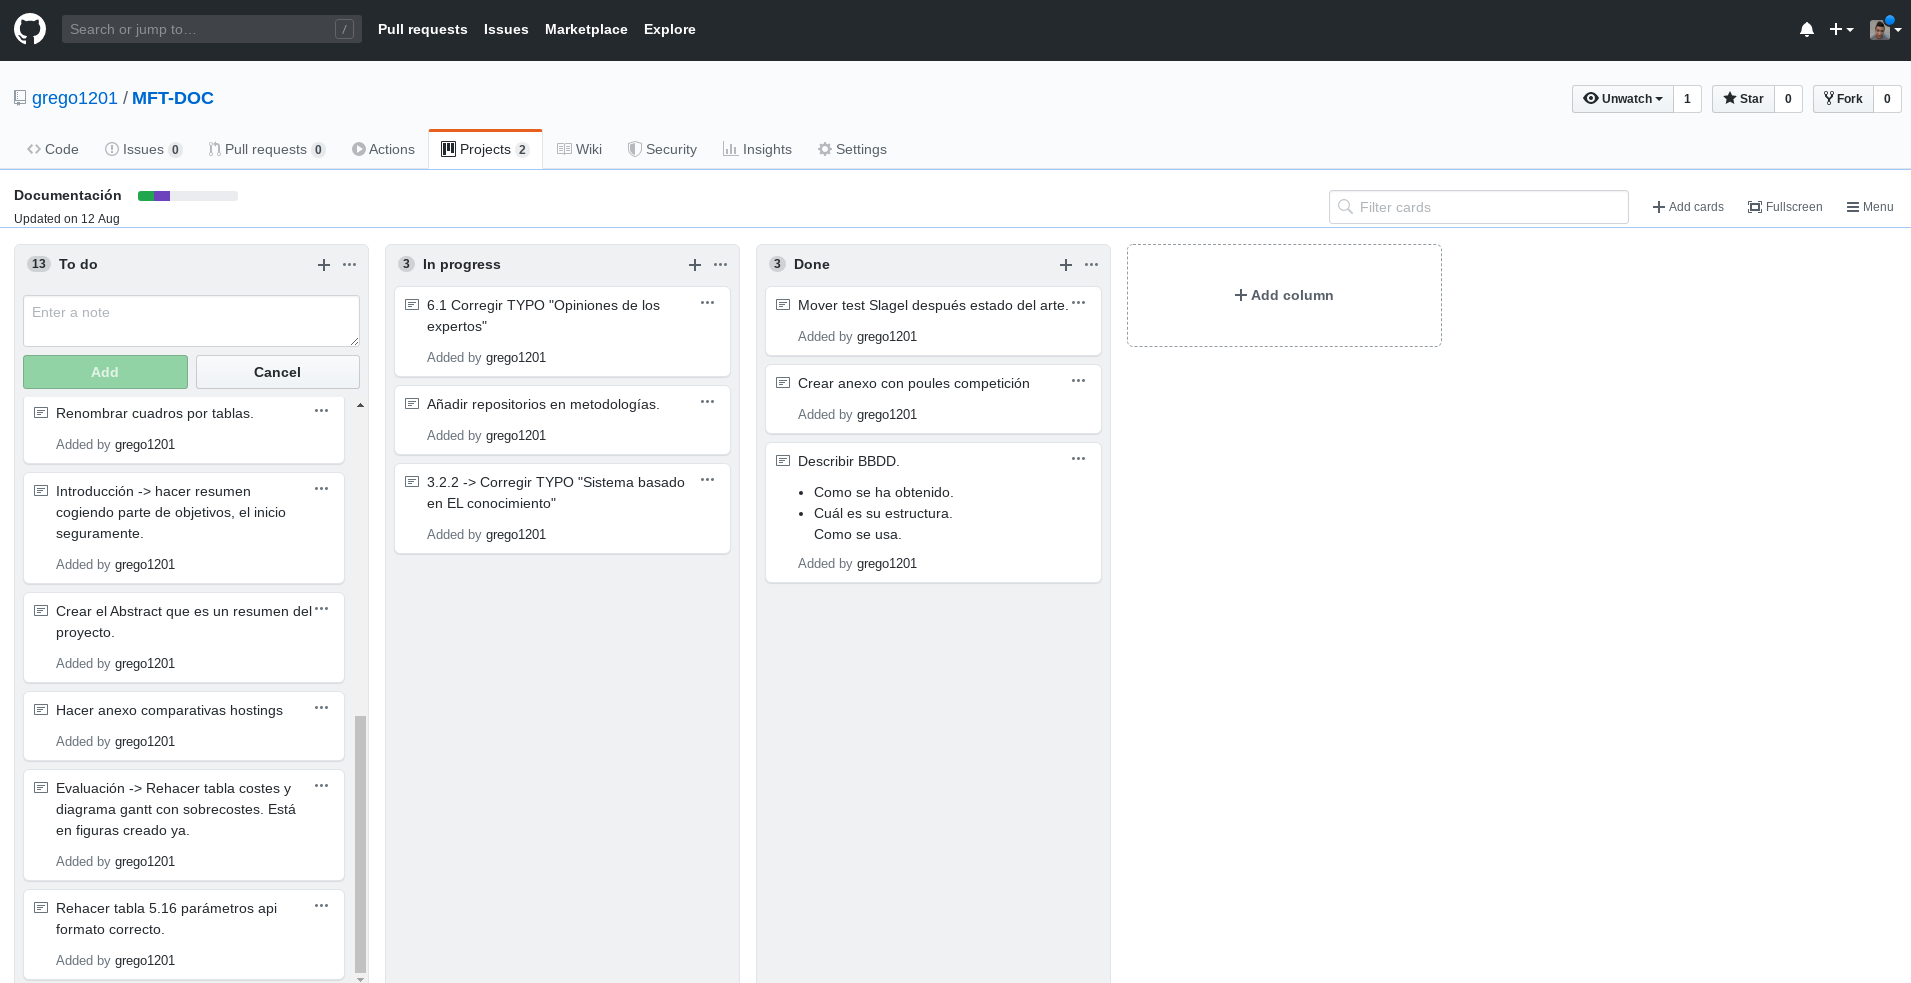
\includegraphics[width=0.9\linewidth]{kanban}
  \caption[Tablero kanban proyecto documentación]{Tablero kanban proyecto documentación}
  \label{fig:Tablero kanban proyecto documentación}
\end{figure}

Un motivo por el que fue elegida esta herramienta es la retroalimentación que brinda ante
el progreso de las tareas. En todo momento se puede saber el número de tareas que tenemos
en cada columna. Además hay un histórico de proyectos. Esto facilitará el cambio de metodología
en un futuro si se quisiera usar SCRUM en vez de XP, pudiendo facilitar
el concepto de sprints\footnote{Sprint: periodo en el cual se realizan tareas. Cada sprint debería tener un objetivo final como por ejemplo terminar una funcionalidad}. El cambio será tan sencillo como crear un proyecto por cada sprint.
El flujo de trabajo será el mismo, el cual será explicado a lo largo de este capítulo.

El tablero elegido fue el básico puesto que el flujo de trabajo no será de gran complejidad.
Como se explicó antes, tendremos tres columnas por las que irán pasando las tareas. Estas serán pequeños progresos y avances que sean requeridos para completar la iteración
que se esté desarrollando. El flujo de trabajo será el siguiente:

\begin{enumerate}
  \item Añadir las tareas a la columna pendiente. Ordenar estas según su orden de prioridad.
  \item Coger la primera tarea de la columna pendiente y moverla a la columna en progreso.
  \item Desarrollar dicha tarea. En caso de existir algún bloqueo y se tenga que esperar,
    se cogerá la siguiente tarea de la columna pendiente.
  \item Una vez finalizada dicha tarea será movida a la columna hecho.
\end{enumerate}

Para evitar la sobrecarga en la columna hecho se archivarán las tareas que lleven dos semanas
en dicha columna. Esto será mas fácil de seguir puesto que al moverlas se hará arriba, en la primera
posición. De este modo cuando se revise habrá que empezar desde la última y estarán todas
ordenadas cronológicamente.

Cada parte del proyecto tendrá su propio tablero para identificar cuales son las necesidades de los mismos.
De este modo tendremos independencia entre ellos y así facilitar la continuidad de los mismos
con un trabajo futuro.

Añadir que además GitHub facilita un sistema de tickets\footnote{Sugerencias sobre cambios o mejoras.}, también conocidos como issues. Con la
configuración correcta estas issues crearán una nueva tarjeta en el tablero kanban correspondiente.
Además, siguiendo un flujo de trabajo de Pull Request\footnote{Pull request: petición que se hace a un proyecto para llevar a cabo un cambio en él.} y, de nuevo, con la configuración adecuada se
podrá automatizar el movimiento de las tareas en nuestro tablero. De este modo se conseguirá la
automatización de todo este proceso ahorrando mucho trabajo y pudiendo centrarnos en analizar los
resultados.
